\documentclass[10pt]{article}
\usepackage[utf8]{inputenc}
\usepackage{float}
\usepackage{url}
\usepackage[portuguese]{babel}
\usepackage{graphicx}
\usepackage{microtype}
\usepackage[T1]{fontenc}

\title{IF755 - REALIDADE VIRTUAL}
\author{Jonathas vinicius }
\date{\vspace{-5ex}}

\usepackage{natbib}

\begin{document}

\maketitle

\section{Introdução}

A disciplina de realidade virtual tem como objetivo fazer com que os discentes aprendam a programar com algumas linguagens especificas para esta areá, nela também se aprende conceitos avançados e ferramentas para VR/AR desenvolvendo a capacidade do aluno para construir tecnologias que suportem o desenvolvimento de VR/AR e seus sistemas tendo aplicações em áreas como jogos,marketing e medicina.

\begin{itemize}
  \item Seus objetivos são fazer com que o discente Conheça conceitos avançados e ferramentas para
\\- Realidade Virtual (VR)
\\ - Realidade Aumentada (AR)
\\ - Desenvolver a capacidade de
\\- Construir tecnologia que suporte o desenvolvimento de VR e / ou AR
sistemas
\\ - Construir soluções inovadoras de RV e / ou AR, focando diversas
domínios de problema .\cite{primeira}
\end{itemize}

A disciplina está inserida na área de MÍDIAS E INTERFACES , sendo o seu profissional é responsável pelo desenvolvimento e criação de programas e sistemas de realidade virtual ou aumentada (VR/AR).

\begin{figure}[]
    \centering
    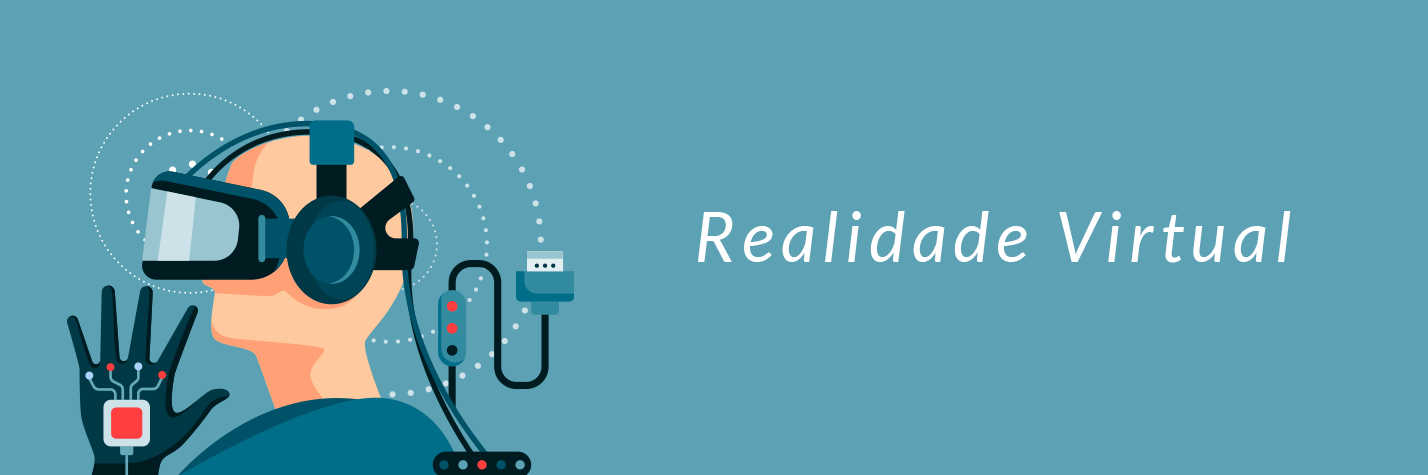
\includegraphics[scale=0.15]{realidadevirtual.png}
    \caption{REALIDADE VIRTUAL \cite{quinta}}
    \label{fig:realidadevirtual}
\end{figure}

\section{Relevância}
Essa cadeira e voltada para pessoas com interesses em computação gráfica, processamento de imagens ou visão computacional.sendo uma inovação e natural que cientistas da computação queiram no currículo por abrir portas para o mundo da tecnologia e do trabalho.\cite{segunda}

\section{Relações}
Algumas disciplinas que são relacionadas com a realidade virtual que estão na grade curricular e o motivo de estarem relacionada.


\begin{tabular}{lllll}
\cline{1-2}
\multicolumn{1}{|l|}{IF681 Interface Usuário Maquina \cite{terceira}} & \multicolumn{1}{l|}{\begin{tabular}[c]{@{}l@{}}Conceitos ainda \\básicos de design \\ de interação e\\  design thinking para a\\  concepção de\\   sistemas \\computacionais interativos.\end{tabular}}                                                            &  &  &  \\ \cline{1-2}
\multicolumn{1}{|l|}{IF687 Introdução à Multimídia \cite{quarta}}   & \multicolumn{1}{l|}{\begin{tabular}[c]{@{}l@{}}Virtual e de aplicações de \\multimídia,\\ desenvolver a capacidade\\ de propor e\\  criar e avaliar mundos \\virtuais, a \\ capacidade de \\especificar, construir\\  e avaliar \\componentes multimídia.\end{tabular}} &  &  &  \\ \cline{1-2}
                                                      &                                                                                                                                                                                                                                                                &  &  &  \\
                                                      &                                                                                                                                                                                                                                                                &  &  & 
\end{tabular}




\bibliographystyle{plain}
\bibliography{jvras}

\end{document}